\section{Resultate}\label{resultate}

\subsection{Lösung 0, Clientseitiges Subsampling auf dem Server ausführen }
5grad
\subsubsection{Artefakte}

\subsection{Lösung 1, Diskrete Kosinus Transformation}
Die Lösung 0 erreicht bereits tiefe Kompressionen. 

\subsubsection{Proof of Concept}
Es gibt unterschiedlichste Wege eine Diskrete Kosinus Transformation zu implementieren. Im Rahmen von diesem Projekt ist es leider nicht möglich alle Wege zu erforschen. Es wird deshalb zuerst mit einem vereinfachten Test ein möglichst vielversprechender Ansatz gesucht, welcher dann im zweiten Schritt komplett ausgearbeitet wird. Mit dem vereinfachten Test sollen folgende Fragen beantwortet werden:
\begin{itemize}
	\item Welches Koordinatensystem soll verwendet werden?
	\item Was für einen Einfluss hat eine Verschiebung der Koordinatenachsen?
	\item Was für einen Einfluss hat die Transformation der Ableitung?
\end{itemize}
Dazu wird nur eine einzige Simulation der Feldlinien verwendet, welche bereits Quantisiert ist. Gemessen wird die Standardabweichung des Radius, Phi und Theta Kanals respektive der X,Y,Z Kanäle. Für den Test wird jeweils eine einfache Quantisierung durchgeführt: Ab dem $128$ Parameter wird alles auf $0$ gesetzt.\\
[\baselineskip]
\textbf{Einfluss der Korrdinatenverschiebung}\\
Der JPEG Standard  benutzt ebenfalls eine Diskrete Kosinus Transformation. Vor der Transformation wird aber der Wertebereich um Null zentriert: Wenn die Eingabepixel einen Wertebereich von  $0$ bis $255$ haben, wird dieser $-128$ bis $127$ verschoben \cite{wiki:dct:jpeg}. Diese Verschiebung soll den ersten Parameter, den DC Koeffizienten \cite{wiki:dc_bias} dämpfen.\\
[\baselineskip]
Im Abschnitt \ref{konzept:ist-komprimierung} wurde bereits der Wertebereich von den Kanälen Radius, Phi und Theta beschrieben. Es ist nochmals darauf hinzuweisen, dass bei der Ist-Quantisierung der Höchstwert auf $2^{15}$ fällt, was beim Signed 16 Bit Integer zu einem Overflow führt, sprich zum Wert $-2^{15}$. Wenn also eine Feldlinie den Längengrad Nullpunkt überschreitet, wird Phi zuerst den Wert $2^{15}-1$ annehmen, dann auf $-2^{15}$ springen und wieder zurück auf 0. Diese Sprünge können sich negativ auswirken. Solche Sprünge können nur mit hochfrequente Anteilen dargestellt werden und sind dadurch schlechter zu komprimieren. Durch eine Verschiebung würde der Phi-Kanal zwar immernoch sprünge beinhalten, wenn der Nullpunkt überschritten wird. Jedoch nur noch von $2^{14}-1$ auf $-2^{14}$.
\begin{figure}[!htbp]
	\center
	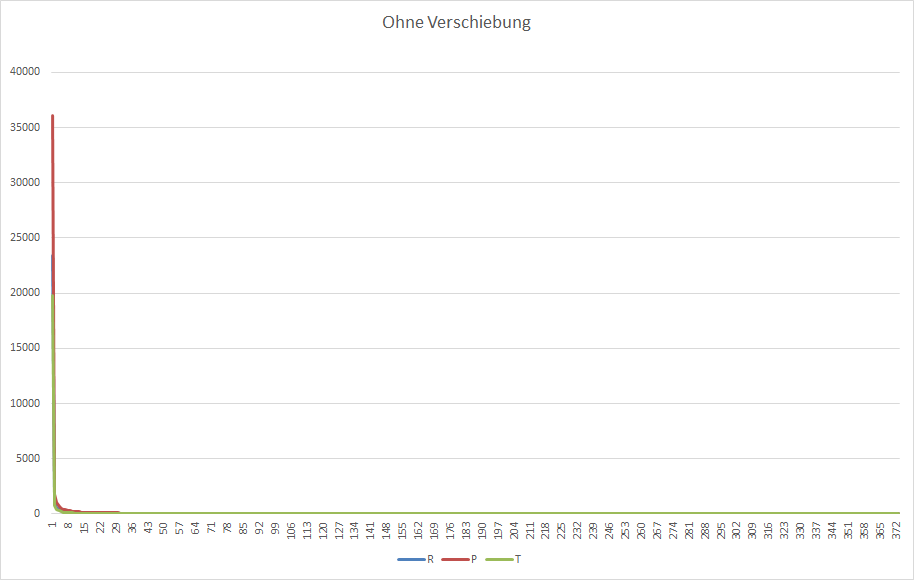
\includegraphics[width=0.4\textwidth,height=6cm,keepaspectratio]{./pictures/resultate/loesung1/spherical_normal.png}
	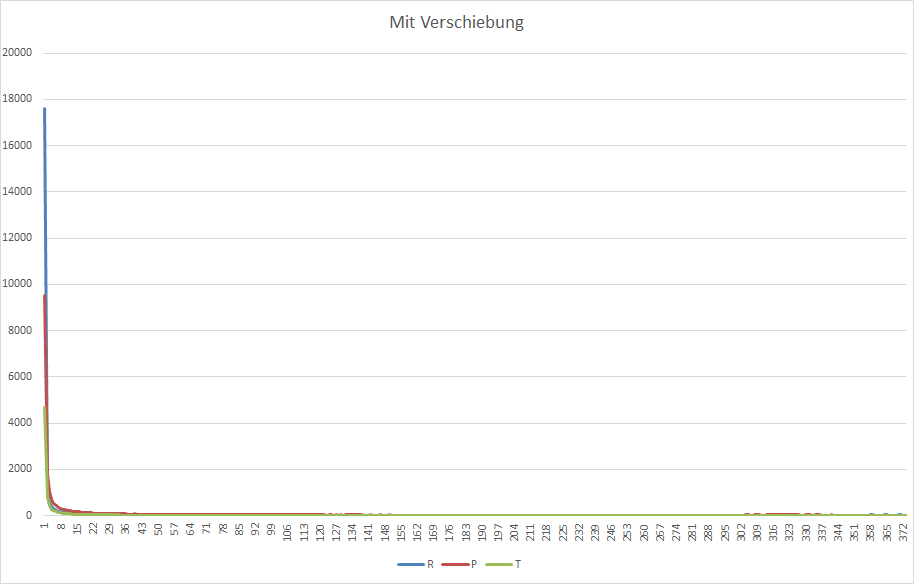
\includegraphics[width=0.4\textwidth,height=6cm,keepaspectratio]{./pictures/resultate/loesung1/spherical_moved.png}
	\caption{Absoluter Median des Resultat der Kosinustransformation. Links ist das Resultat der sphärischen Koordinaten. Rechts das Resultat der um den Nullpunkt zentrierten Koordinaten.}
	\label{resultate:loesung1:poc:wertebereich}
\end{figure} 
\begin{table}[!htbp]
\center
	\begin{tabular}{l|c|c}
	 Kanäle & Std. Abw. Normal &  Std. Abw. zentrierten Koordinaten\\\hline
	 Radius & 124.397 & 124.316\\
	 Phi & 1236.350 & 256.565\\
	 Theta & 83.723 & 83.527\\
	\end{tabular}
	\caption{Vergleich der Standardabweichung pro Kanal. Die Werte sind im diskretisierten sphärischen Koordinatensystem}
	\label{resultate:loesung1:poc:wertebereich_tabelle}
\end{table}
In der Abbildung \ref{resultate:loesung1:poc:wertebereich} ist deutlich zu sehen, dass der DCT Koeffizient im Vergleich gedämpft wurde. Das bedeutet, dass bei einer späteren Quantisierung der DCT Koeffizient mit weniger Präzision abgespeichert werden kann, ohne einen hohen Fehler zu verursachen.\\
Die Tabelle \ref{resultate:loesung1:poc:wertebereich_tabelle} zeigt deutlich, dass dank der Koordinatenverschiebung der Phi-Kanal etwa vier Mal genauer dargestellt werden kann. Vermutlich ist es den verkleinerten Sprüngen zu verdanken, wenn eine Kurve den Nullpunkt überschreitet.\\
[\baselineskip]
\textbf{Einfluss der Ableitung}\\
Warum Ableitung: kleinere parameter,
\begin{figure}[!htbp]
	\center
	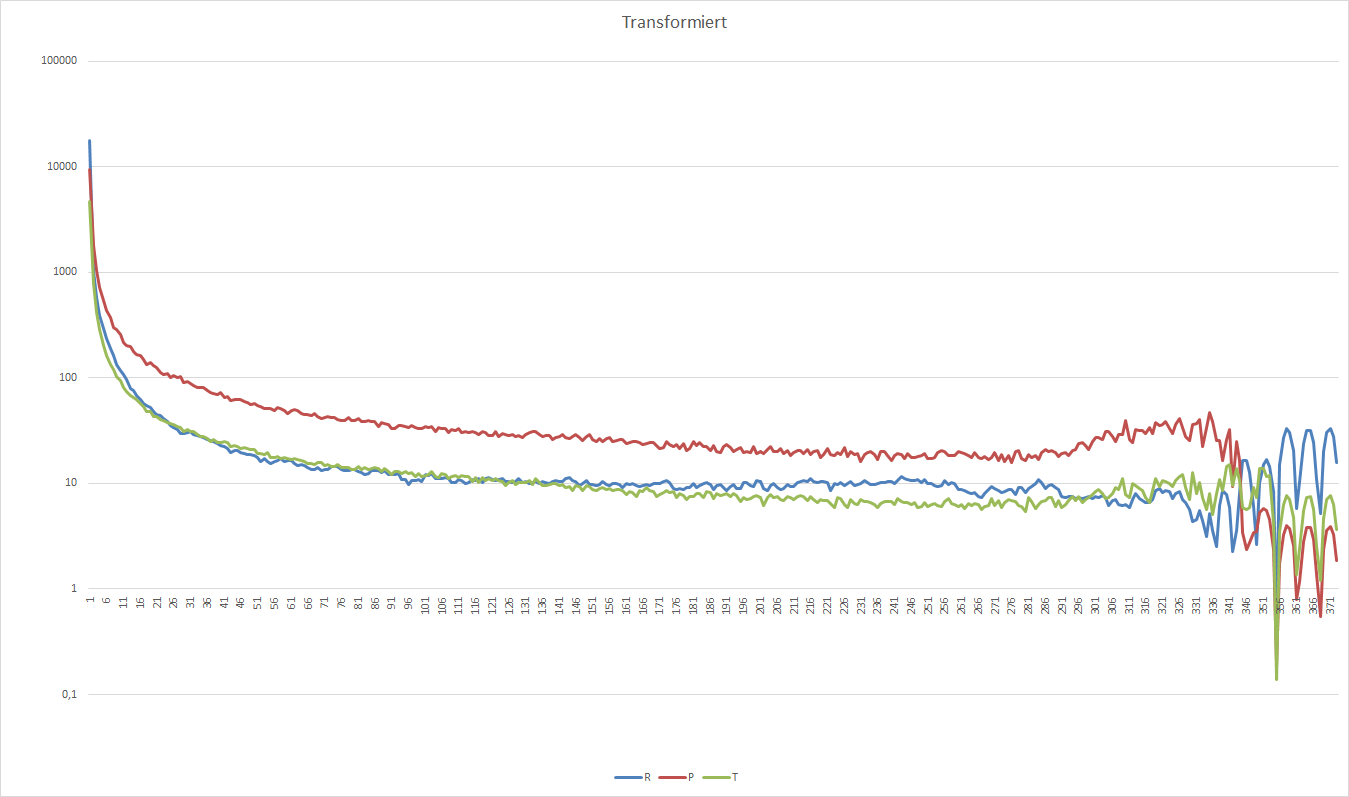
\includegraphics[width=0.4\textwidth,height=6cm,keepaspectratio]{./pictures/resultate/loesung1/spherical_log.png}
	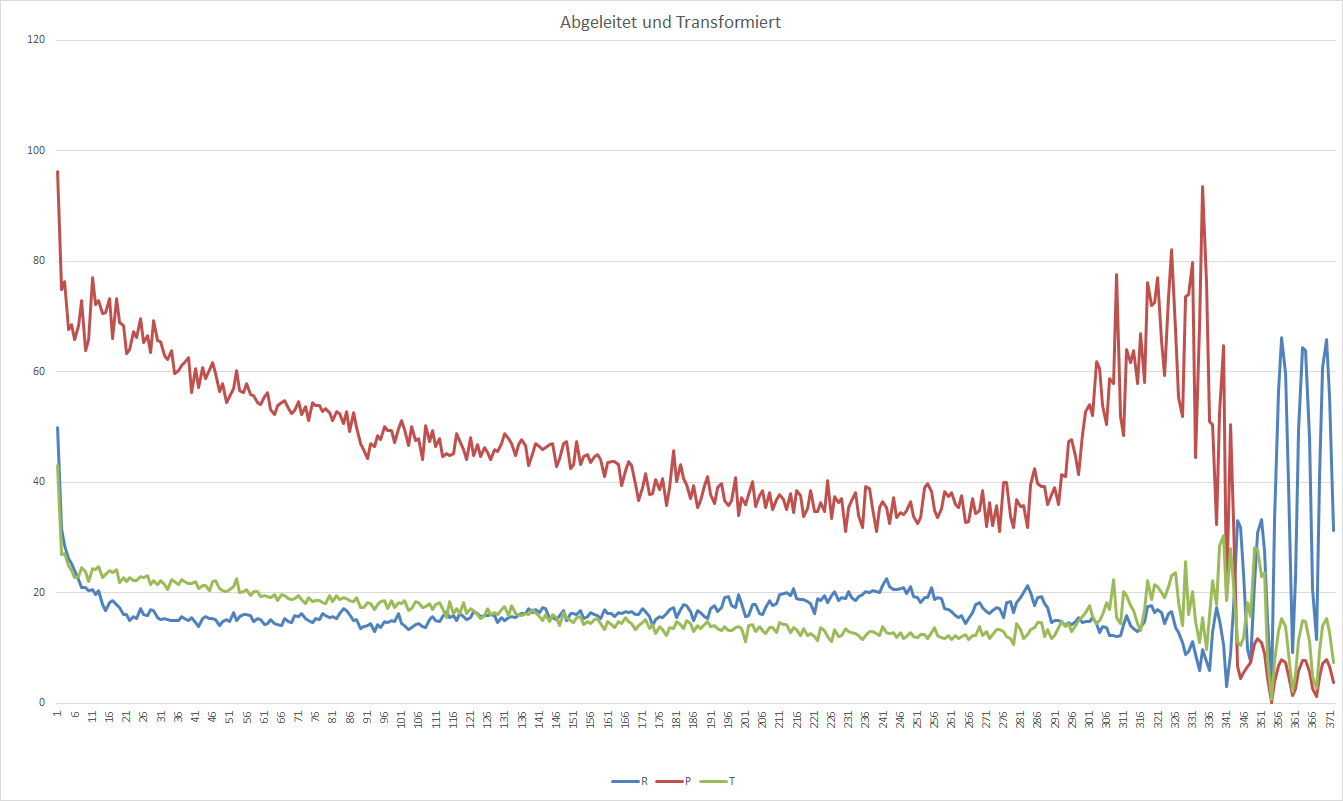
\includegraphics[width=0.4\textwidth,height=6cm,keepaspectratio]{./pictures/resultate/loesung1/spherical_dt.png}
	\caption{Absoluter Median des Resultat der Kosinustransformation. Links ist das Resultat der um den Nullpunkt zentrierten Koordinaten auf einer logarithmischen Skala. Rechts das Resultat der Ableitung auf einer linearen Skala.}
	\label{resultate:loesung1:poc:ableitung}
\end{figure} 
\begin{table}[!htbp]
\center
	\begin{tabular}{l|c|c}
	 Kanäle & Std. Abw. zentrierten Koordinaten &  Std. Abw. der Ableitung\\\hline
	 Radius & 124.316 & 124.135\\
	 Phi & 256.565 & 256.084\\
	 Theta & 83.527 & 83.723\\
	\end{tabular}
	\caption{Vergleich der Standardabweichung pro Kanal. Die Werte sind im diskretisierten sphärischen Koordinatensystem}
	\label{resultate:loesung1:poc:ableitung_tabelle}
\end{table}
Resultat: Dämpfung der Parameter, aber
Keine bessere Genauigkeit.
Aber sachverhalt repeat:
\begin{table}[!htbp]
\center
	\begin{tabular}{l|c|c}
	 Kanäle & Std. Abw. der Ableitung &  Std. Abw. bei Parameterwiederholung\\\hline
	 Radius & 124.135 & 94.879\\
	 Phi & 256.0845 & 228.332\\
	 Theta &  83.723 & 67.667\\
	\end{tabular}
	\caption{Vergleich der Standardabweichung pro Kanal. Die Werte sind im diskretisierten sphärischen Koordinatensystem}
	\label{resultate:loesung1:poc:repeat_tabelle}
\end{table}

repeat wirkt sich positiv auf die Genauigkeit aus. Es besteht die Möglichkeit die DCT zu approximieren mit anderen Funktionen?\\
[\baselineskip]
\textbf{Auswahl des Koordinatensystems}

Warum Sphärisch: Kleinere Koeffizienten.
Warum Euklidisch: Kein Wrap-around.
Messung: Nach der Dekompresssion rücktransformation auf euklidische Koordinaten und vergleichen.

Euklidisch Quantisierung auf shorts, ergebnis: Tabelle
\begin{table}[!htbp]
\center
	\begin{tabular}{l|c|c}
	 Kanäle & Std. Abw. sphärische Koordinaten &  Std. Abw. euklidische Koordinaten\\\hline
	 X (Meter) & 43551184 & 27087946\\
	 Y (Meter) & 19656055 & 17154731\\
	 Z (Meter) & 40825926 & 26242294\\
	\end{tabular}
	\caption{Vergleich der Standardabweichung pro Kanal.}
	\label{resultate:loesung1:poc:koordinatensysteme}
\end{table}

\subsubsection{Implementation}
Residuals + Speicherung
Subsampling da Punktmenge zu gross
Erster Versuch speicherung:





Fehler mit Diskretisierung

\textbf{Kann das Client Subsapmling verwendet werden}
5grad währe schön, viel kleinere Punktmenge, aber nicht konstante Abstände

\subsubsection{Artefakte}
2D Feldlinie zeigen, normal und komprimiert
